\chapter{Planificación}

\section{Metodología utilizada}

Para el desarrollo de este proyecto se ha elegido como metodología el \textbf{Desarrollo Ágil}.
En mi opinión, este tipo de enfoque se acerca más al que desarrollan las empresas en la actualidad, donde se
definen sprints en los que los requisitos y soluciones van evolucionando según la necesidad del proyecto.
No obstante cada iteración deberá tener su planificación, análisis de requisitos, diseño, tests, etc.

\section{Temporización}

La temporización general de este proyecto va a estar dividida en dos: construcción del Web Service para la
gestión de los datos del aplicativo y la creación de un entorno Front-End para los usuarios. A su vez estos dos
objetivos principales estarán divididos en diferentes hitos para realizar un desarrollo progresivo.

\vspace{0.5em}
\begin{itemize}
    \item \textbf{Web Service}:
        \begin{itemize}
            \item \textbf{Gestión de citas previas}: En este primer hito se completará toda la funcionalidad referente
            a la gestión de cita previa. Contendrá todo lo necesario para que desde la aplicación Webs se puedan
            realizar operaciones como reserva de citas por parte de usuarios; obtención de histórico de citas ya
            sea del negocio, usuarios o trabajadores; cancelación de citas; así como todas las comprobaciones y
            controles para la gestión de estas citas. De la mano de este hito se completará también la gestión
            de inicio de sesión de usuario y la encriptación de datos privados en la base de datos del aplicativo.

            \item \textbf{Integración Continua}: Este hito no hace aportación de nueva funcionalidad
            para el Web Service en construcción pero si es una parte esencial del proyecto. El objetivo
            es poder tener una batería de test para la aplicación y mediante
            Github Actions, que será el Sistema de Integración Continua elegido, lanzar estos tests en los commits
            que se vayan realizando en el desarrollo del proyecto. Así nos aseguraremos que en toda nueva funcionalidad
            creada o mejoras de código se realizan las acciones deseadas.

            \item \textbf{Gestión de venta de productos online}: Una vez finalizadas las dos etapas anteriores
            pasaremos a desarrollar otro de los puntos principales del problema, la gestión de venta online de
            productos. En este hito se deberá implementar la gestión de los pedidos que lleguen desde la aplicación
            Front-End de los usuarios de las Webs.

            \item \textbf{Administración Back-End}: Por último se va a añadir para el Back-End desarrollado una vista
            de administración para poder acceder a todos los datos registrados por cada negocio. Además se podrán
            añadir funcionalidades para los trabajadores o un panel de estadísticas donde ver información relevante.
        \end{itemize}
    \item \textbf{Aplicación Web/Móvil}:
    \begin{itemize}
                \item \textbf{Esqueleto y Home}: El primer hito correspondiente al desarrollo Front-End del aplicativo
                será la construcción del esqueleto Web (header, barra de navegación, footer, etc.) Junto con la Home
                con información y presentación del negocio.

                \item \textbf{Interfaz para la reserva de citas}: Una vez cumplido el primer hito pasaremos al
                desarrollo de lo referente a las citas previas. Se creará una vista donde ver las citas disponibles del
                negocio y poder reservarlas como usuario autenticado, además de una vista individual donde ver
                un histórico de citas reservadas y próximas citas.

                \item \textbf{Interfaz para las compras online de productos}: Por último finalizaremos este trabajo con
                el desarrollo de la interfaz para la tienda online. Se creará una vista donde se muestren los productos
                del negocio con los filtros correspondientes para los productos. Se podrán añadir productos al carrito
                de compra y realizar el pago de los productos deseados para realizar los pedidos.

            \end{itemize}
\end{itemize}
\subsection{Sprint definidos}

Además de la organización para el desarrollo del sistema, también se debe organizar el tiempo a invertir para el análisis previo necesario y el diseño de base de datos o interfaces de la aplicación. Una vez tengamos todos los puntos estudiados y definidos podremos comenzar con el desarrollo en programación. Podemos ver la organización prevista en la siguiente imagen:


\begin{figure}[H]
  \centering
  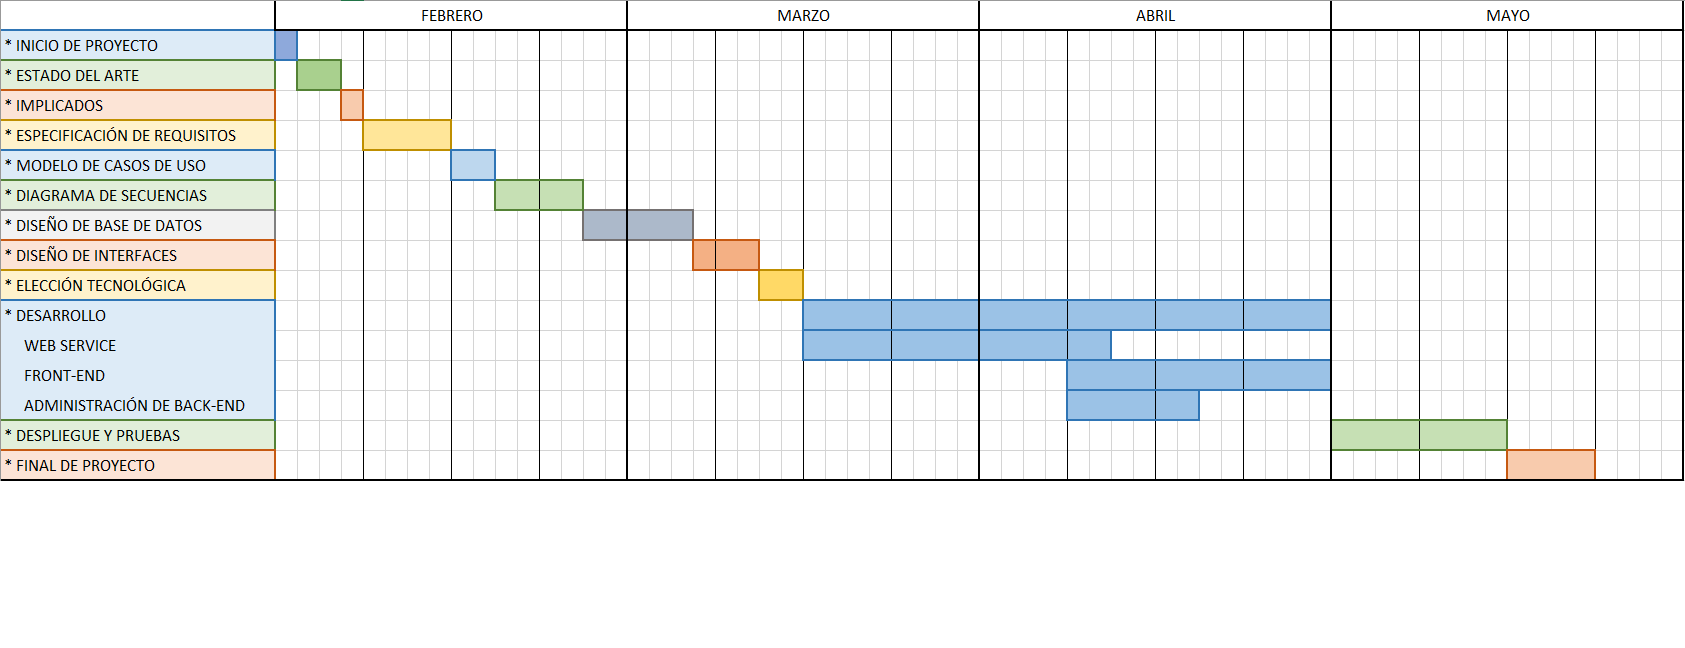
\includegraphics[scale=0.27]{images/Sprint_Prevision.png}
  \caption{Previsión de sprint a desarrollar}
  \label{}
\end{figure}

Como se indica, el tiempo transcurrido desde que se comienza este proyecto hasta que se pasa a la parte de desarrollo web es de aproximadamente mes y medio. Esto es debido a la cantidad de información y casuisticas que debemos analizar. Además el análisis previo es muy importante a la hora del diseño de la base de datos ya que a partir de este obtendremos toda la información necesaria de almacenar y las relaciones que tendremos entre nuestras entidades.

La programación ocupará tamién alrededor de un mes y medio de trabajo. Con todo el analisis y diseño ya realizado no debería llevar un tiempo muy prologado su implementación, aunque siempre podemos encontrarnos problemas de integración con herramientas externas que utilicemos.

Por último tendremos dos semanas para el despliegue en producción y pruebas para comprobar que todo funciona perfectamente.